\section{Implementation}\label{sec:chapter-6}

\subsection{Mobile application and state management}

The mobile source separates screens, services, shared types, navigation, context, and theme definitions. Authentication context manages account state, journal context coordinates unlock and entry operations, and audio-player context supports playback across screens. Service modules centralise API access rather than embedding every network request in presentation components. This structure helps changes such as a new journal envelope format propagate through a defined layer while preserving the screen's writing interaction.

The application includes dedicated authentication and account-security screens, multi-step check-in components, exercise detail and playback, free writing, prompted journaling, course navigation, and PDF viewing. Recent source also includes journal attachment composition and media handling. Their existence is implementation evidence, but the earlier documented simulator checks should not be stretched to cover every later attachment path. The report therefore treats the wider media feature set as source-observed capability requiring release-level verification.

\begin{figure}[htbp]
\centering

\includegraphics[width=\linewidth,height=0.62\textheight,keepaspectratio]{figures/library.png}
\caption[Library screen]{Existing iOS simulator Library screen, captured 3 October 2026. Course progress and the persistent compact audio player demonstrate implemented presentation features.}
\label{fig:library}
\end{figure}
\FloatBarrier

\subsection{Authentication and persistence}

The backend owns account identity and stores private records under that identity. Passwords are hashed, session storage uses native secure storage, and authenticated routes apply account-specific queries. Email verification, password recovery, password change, and account deletion have dedicated flows. Google identity-token verification is present in source, with native and backend configuration requirements. Apple identity handling remains for compatibility, while its sign-in controls were removed from the mobile authentication screens on 3 October 2026. Current provider implementation does not establish a completed production-signed login test.

PostgreSQL separates structured data from hosted media. Onboarding supplies a support goal, check-ins supply present context, and recommendation requests record returned items and associated context. Feedback and event records retain evidence for later adaptation. Persistence is especially important across app restarts, but it also introduces retention and deletion responsibilities. Account deletion can remove server-linked records and attempt local-key cleanup; it cannot erase a recovery key copied elsewhere or material retained outside the application's control.

\subsection{Five-stage hybrid recommendation engine}

The Node recommendation route loads onboarding, the latest check-in, eligible published exercise records, interaction aggregates, discomfort exclusions, and recent recommendation IDs. It rejects generation when required context is unavailable. User identifiers are transformed with an HMAC before being sent to the Python service. This reduces direct identifier exposure across that boundary, but the transformed identifier still links interactions within the service. Pseudonymisation is therefore not equivalent to anonymous data.

The Python engine loads its tokenizer and ONNX model, truncates input at the configured limit, pools token outputs when needed, and normalises embeddings. Scoring records component values and returns an explanatory reason. Collaborative activation requires at least two qualifying neighbours and at least two common interactions under current defaults. Without those conditions, the engine labels its strategy as content-based cold start. The saved benchmark exercises this cold-start pathway and cannot support conclusions about collaborative quality.

The application also has a local fallback recommendation algorithm for service failure. It shares comfort mapping with backend policy, but it is a different ranker from the Python benchmark. A successful empty response is preserved rather than refilled with unfiltered local suggestions. This distinction is important: degraded operation may justify alternate ranking, while an empty eligible set should continue to communicate that no suitable items were available under current constraints.

The interaction aggregation also deserves scrutiny. Current backend code combines explicit feedback and event values over a bounded recent period, groups them by user and exercise, and limits the returned interaction dataset. Averaging is simple to inspect, but may suppress disagreement between a completed activity and an uncomfortable experience. Sparse observations, repeated clicks, and differences in how users provide ratings can distort neighbour similarity. Future analysis should examine these behaviours before adjusting weights or increasing the influence of collaboration. A pseudonymous identifier helps separate the service from direct account identifiers, but does not remove the sensitivity of the behavioural record.

\subsubsection{Pipeline overview and service integration}
\label{sec:five-stages}

The project's recommendation workflow has five logical stages: (1) eligibility filtering, (2) suitability rules, (3) semantic matching, (4) collaborative signals, and (5) final ranking and explanation. These stages describe responsibilities rather than five independently deployed services. The Node API constructs the request and the Python service implements filtering and ranking. Within \texttt{recommend()}, vector encoding and neighbour estimation are calculated before the per-item score loop; the stage numbering below is an explanatory decomposition of that function, not a claim about its literal line-by-line execution order. Figure~\ref{fig:recommendation-five-stages} connects these responsibilities to the feedback loop.

\subsubsection{Stage 1: construct and filter the eligible candidate set}
\label{sec:stage-one}

The authenticated API loads the latest check-in, onboarding support goal, published recommendation-enabled exercises, behavioural aggregates, discomfort exclusions, and recent recommendation identifiers. A missing check-in produces an HTTP~409 response; an empty published catalogue produces HTTP~503. The API does not accept a client-supplied account identifier as authority for accessing private context. It converts identifiers to HMAC-SHA256 pseudonyms before the Python request. The current request explicitly contains \texttt{journal\_texts: []}; neither journal plaintext nor journal embeddings are uploaded for ranking.

The check-in supplies six dimensions: state, body, energy, stress, focus, and support. Optional comfort choices are mapped through a shared policy. Self-touch avoidance excludes the butterfly hug and self-containment hold; breath-hold avoidance excludes box breathing and candidates marked as requiring holds; head/eye scanning avoidance excludes orienting; inward body-scan avoidance excludes body scanning. These restrictions belong to the latest check-in. Separately, exercises previously reported as uncomfortable are excluded through account-specific feedback records.

Python's \texttt{eligible\_candidates()} deduplicates IDs, removes the explicit exclusion set, and applies \texttt{contraindication\_reasons()}. Signals are normalised before comparison with metadata. The existing high-activation policy removes breath-hold exercises when the reported state is anxious or overwhelmed, or stress is very stressed. These are implemented suitability policies, whose completeness depends on the declared inputs and content metadata. They are not an automated clinical assessment.

Let $E$ be the published candidate set, $X_u$ the explicit and discomfort-derived exclusions, and $Q(e,u)$ the implemented metadata/high-activation rejection predicate. The eligible set is
\begin{equation}
 E_u = \{e\in E: e\notin X_u \text{ and } \neg Q(e,u)\}.
 \label{eq:eligibility}
\end{equation}
Only $E_u$ proceeds to scoring and fresh-item selection. An exercise cannot regain eligibility through a high embedding score, a positive peer rating, or a need to fill four slots. If $E_u$ is empty, the engine returns an empty list with \texttt{no-candidates}. This is a valid policy outcome rather than an instruction to relax restrictions.

\subsubsection{Stage 2: calculate structured suitability rules}
\label{sec:stage-two}

\texttt{\_rule\_evaluation()} compares normalised check-in answers with an exercise's recommendation tags, support goals, and intended states. The field contributions are support~0.34, state~0.22, body~0.12, energy~0.10, stress~0.10, and focus~0.08. They sum to~0.96; they are not a probability distribution. Additional adjustments consider activation level and physical intensity. For example, a down-regulating exercise receives~0.12 for a calm-down support match and~0.10 for an anxious/overwhelmed state. Up-regulating activities receive~0.14 for an energy support match. High-intensity activity is penalised by~0.38 for tired/drained energy; moderate intensity is penalised by~0.10 in that condition. The resulting rule score is clipped to $[0,1]$.

Writing $m_j(e,u)$ for a metadata match in field $j$, $w_j$ for its contribution, and $\Delta(e,u)$ for the implemented adjustments gives
\begin{equation}
 R(e,u)=\operatorname{clip}_{[0,1]}\!\left(\sum_j w_jm_j(e,u)+\Delta(e,u)\right).
 \label{eq:rule-score}
\end{equation}
Hard eligibility and soft ranking adjustments have distinct purposes. A metadata contraindication causes removal in Stage~1; a moderate-intensity penalty can instead reorder otherwise eligible items. The returned matched fields also support explanation text. These transparent heuristics are defensible as inspectable implementation choices, but the present benchmark does not independently validate every weight or suitability interpretation.

\subsubsection{Stage 3: compare meaning using MiniLM embeddings}
\label{sec:stage-three}

The engine constructs three kinds of document: the current check-in context, the goal/history context, and one description per eligible exercise. Exercise descriptions concatenate title, category, description, recommendation tags, support goals, intended states, activation level, and intensity. The current context uses labelled check-in answers. Although the Python schema retains a history-document function for older evaluation fixtures, the current application supplies no journals; the live history component uses the onboarding goal when present.

The pretrained \texttt{all-MiniLM-L6-v2} tokenizer truncates inputs at 256 tokens. ONNX Runtime executes the model on the CPU. When inference returns token-level vectors, attention-mask-weighted mean pooling excludes padding; sentence-level outputs are used directly. Embeddings are converted to NumPy arrays, checked for expected shape, and normalised. Current-context similarity $C$ and goal/history similarity $H$ use the clipped cosine comparison
\begin{equation}
 C(e,u)=\operatorname{clip}_{[0,1]}\!\left(\frac{\mathbf v_e\cdot\mathbf v_c}{\|\mathbf v_e\|\,\|\mathbf v_c\|}\right),\qquad
 H(e,u)=\operatorname{clip}_{[0,1]}\!\left(\frac{\mathbf v_e\cdot\mathbf v_h}{\|\mathbf v_e\|\,\|\mathbf v_h\|}\right).
 \label{eq:semantic-score}
\end{equation}
If the goal/history document is empty, the code still encodes that document; it does not explicitly disable the five-percent history term. This is a concrete implementation limitation worth considering in a future ablation. The model is pretrained rather than trained or fine-tuned on the project's users. It measures descriptive similarity and does not generate therapeutic advice.

If model loading or inference fails, production Python can use deterministic, 384-dimensional hashed token counts. SHA256 assigns tokens to dimensions, after which vectors are normalised. This lexical fallback is labelled in the model backend and logs the error class without user text. Strict ONNX evaluation disables fallback, so a failed model cannot silently produce a benchmark described as semantic inference. The separate mobile fallback is another algorithm and should not inherit the measured accuracy of the Python ranker.

\subsubsection{Stage 4: add collaborative evidence only when sufficient history exists}
\label{sec:stage-four}

The API maps exercise events to bounded preference values: opened~0.15, started~0.35, completed~0.80, saved~0.70, repeated~1.00, and abandoned~$-0.40$. Explicit feedback takes precedence within its own record: uncomfortable maps to~$-1.00$; worse to~$-0.75$; better to~$1.00$; otherwise helpfulness $h\in\{0,1,2,3\}$ maps to $h/1.5-1$. The backend averages combined feedback/event observations per user and exercise over 180 days, clips to $[-1,1]$, and retrieves at most 10,000 aggregate rows. The feedback and event records can therefore counterbalance one another. An uncomfortable exercise nevertheless remains an explicit exclusion for that account, regardless of its averaged value.

User--user cosine similarity is calculated only over jointly interacted exercise IDs. A qualifying neighbour must have at least two common items and positive cosine similarity. At least two qualifying neighbours activate collaboration under the defaults. For an eligible exercise, the component is
\begin{equation}
 B(e,u)=\frac{1}{2}\left(1+\frac{\sum_{v\in N_u(e)}\operatorname{sim}(u,v)r_{v,e}}{\sum_{v\in N_u(e)}\operatorname{sim}(u,v)}\right),
 \label{eq:collaborative-score}
\end{equation}
where $N_u(e)$ contains qualifying neighbours with an observation for $e$. A missing collaborative estimate defaults to~0.5 when collaboration is active. Without enough neighbours, the collaborative contribution is disabled and the returned strategy is \texttt{content-based-cold-start}. This allows a new user to receive suggestions from current context and content metadata.

Feedback changes future inputs; it does not retrain MiniLM after every event. Moreover, a completion event can reflect persistence rather than helpfulness, and two positive-similarity neighbours provide limited evidence. The current saved benchmark has no interaction histories and therefore tests the cold-start path, not the accuracy or fairness of collaborative recommendations.

\subsubsection{Stage 5: blend, rotate, diversify, explain, and persist}
\label{sec:stage-five}

The base blend switches according to collaborative availability:
\begin{align}
 S_{\mathrm{cold}}(e,u)&=0.72R+0.23C+0.05H,\label{eq:cold-start}\\
 S_{\mathrm{warm}}(e,u)&=0.65R+0.20C+0.05H+0.10B.\label{eq:warm-start}
\end{align}
Figure~\ref{fig:recommendation-weights} shows both modes. An earlier diagram's single 65/25/10 split combines current and goal/history similarity and describes only the collaboration-active blend. It does not represent cold-start weights. The revised account separates both semantic terms and both modes.

\begin{figure}[htbp]
\centering
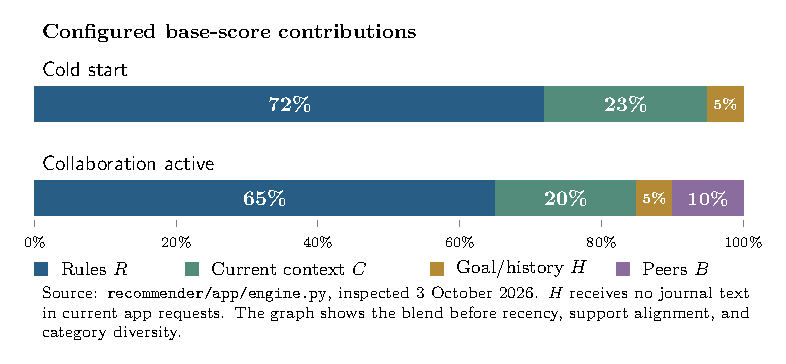
\includegraphics[width=\linewidth,height=0.62\textheight,keepaspectratio]{figures/recommendation-weights.pdf}
\caption[Cold-start and collaboration-active score weights]{Implemented score-component weights in cold start and collaboration-active mode. These are configured ranking contributions, not measured causal importance or success probabilities.}
\label{fig:recommendation-weights}
\end{figure}
\FloatBarrier

The API supplies up to 24 recent item impressions from a 14-day window, excluding requests tied to the same latest check-in. Python approximates request age by each item's index divided by the requested list size. Each impression contributes $0.18\times0.72^a$, with accumulated penalty capped at~0.42. The preselection score is $\max(0,S-P_{\mathrm{recency}})$. This provides gentle rotation, although reconstructing age from item order is approximate when historical lists are shorter than four.

Candidate ordering begins with descending score and exercise-ID tie breaking. If at least four eligible items align with the primary support goal, selection restricts to that pool; otherwise the full eligible set remains available. If enough candidates have recency penalties below $0.9\times0.42$, that less-exposed pool is preferred. Greedy selection then maximises the stored score minus~0.08 for each already selected item in the same category. Category diversity therefore affects positions, but the stored score does not include this per-selection diversity subtraction.

If a complete selected set would repeat the most recent set, only the final slot may be replaced with an unseen, eligible, support-aligned item. That item is marked as exploration. No separate minimum semantic-similarity threshold is enforced in this substitution, so its appropriateness still needs longitudinal evaluation. Normal results contain up to four exercises, score components, reasons, and the exploration flag. Reasons follow deterministic matched-field templates; they explain a declared match and do not provide a complete attribution of every score contribution.

The Node API saves the request, context flags, ordered items, and impression events within a database transaction. Ownership checks govern subsequent feedback. The Home screen maps returned IDs to mobile-renderable exercises and ignores unmapped IDs, another reason fewer than four cards can appear. A successful empty response is preserved. A request failure activates the local TypeScript ranker, which shares comfort filtering but does not receive the server's full persistent discomfort, collaborative, or recency history.

\subsubsection{Worked scoring example and algorithm summary}
\label{sec:worked-recommendation}

Consider an illustrative eligible grounding exercise with $R=0.80$, $C=0.60$, and $H=0.40$. Its cold-start base score is $0.72(0.80)+0.23(0.60)+0.05(0.40)=0.734$. One newest-request impression subtracts~0.18, producing~0.554. If a category peer has already been selected, its selection utility becomes~0.474 after the diversity deduction, while the recorded score remains~0.554. These inputs are deliberately illustrative and are not a measured user case. If the same exercise were explicitly excluded in Stage~1, none of these calculations could return it.

\begin{lstlisting}[caption={Five-stage algorithm summary. Operational logging and ownership checks occur in the API around this ranker.},label={lst:five-stage-algorithm}]
1  context <- authenticated check-in, goal, catalogue, activity
2  eligible <- deduplicate and apply all known exclusions
3  if eligible is empty: return an empty result
4  R <- structured suitability for each eligible exercise
5  C, H <- semantic similarities; journals remain absent
6  B, active <- positive neighbours with sufficient overlap
7  S <- cold blend, or warm blend when active
8  subtract recency; prefer support-aligned eligible options
9  greedily diversify; conditionally replace only final slot
10 return up to four items with reasons and components
11 persist request/items/impressions; accept owned feedback
\end{lstlisting}

The explanation is grounded in \path{backend/src/routes/recommendations.ts}, \path{backend/src/data/comfortPreferences.ts}, \path{recommender/app/engine.py}, \path{src/services/recommendations/recommendationEngine.ts}, and \path{src/screens/home/HomeScreen.tsx}, inspected on 3 October 2026. Equations~\ref{eq:eligibility}--\ref{eq:warm-start} express implemented operations; future weight tuning, independent content review, and collaborative evaluation remain research tasks.


\subsection{Encrypted journaling}

Journal creation begins with vault setup and recovery-backup confirmation. Entry titles, prompts, packs, and text are serialised and encrypted locally. The backend accepts versioned ciphertext envelopes and rejects new plaintext writes. On retrieval, the device decrypts content only after unlocking. Wrong-account, wrong-key, altered-ciphertext, and identifier mismatches should fail authentication rather than display plausible corrupted text. Current source also defines authenticated encryption for journal media, with its own associated identifiers and media purpose.

\begin{figure}[htbp]
\centering
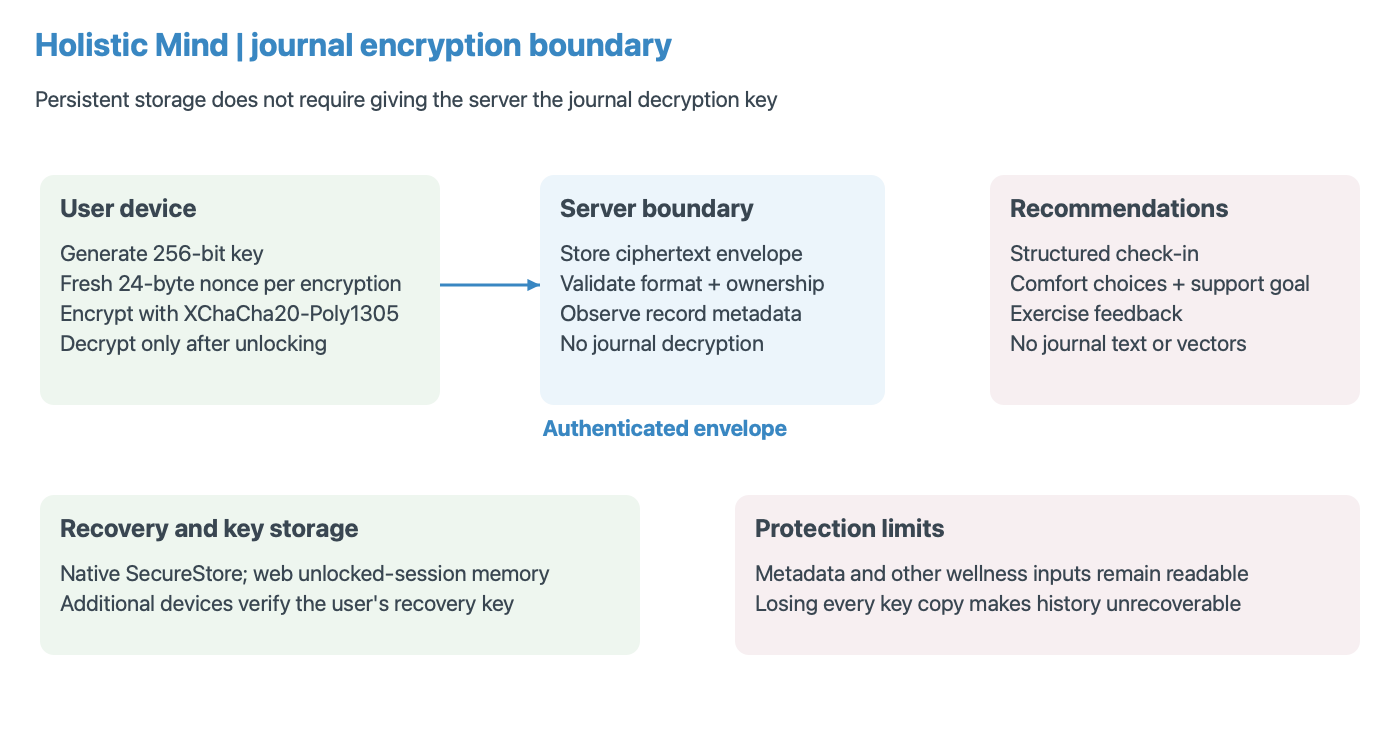
\includegraphics[width=\linewidth,height=0.62\textheight,keepaspectratio]{figures/privacy.png}
\caption[Journal encryption and recovery boundary]{Journal encryption and recovery boundary. The server stores envelopes and metadata; journal text and decryption keys are excluded from recommendation requests.}
\label{fig:privacy}
\end{figure}
\FloatBarrier

Legacy migration is explicit rather than a silent server-side conversion. An unlocked client retrieves older entries, encrypts and verifies them, and submits conditional replacements. The previous plaintext fields become null while the original record identity and timestamp remain. Retrying a migration should return the already encrypted result without overwriting it. The documented tests used synthetic entries and did not migrate real journals. A production transition must also address retained backups and compatibility with older clients.

\subsection{Content administration and deployment}

The administration application manages exercises, audio records, curriculum structure, and related media through protected backend operations. Published status controls ordinary content availability, while recommendation metadata adds intended states, support goals, activation levels, and restrictions. This allows presentation content and ranking semantics to evolve together. However, inaccurate metadata can undermine eligibility even when upload, authentication, and publication mechanisms operate correctly. Content review is consequently part of maintaining recommendation quality.

Local development uses containerised PostgreSQL, object storage, and the recommendation service alongside the API and mobile tooling. Deployment documentation describes managed database, private service networking, S3-compatible hosting, and configured email delivery. These are reproducible operational arrangements, not evidence of full production acceptance. Export/\allowbreak{}import scripts support moving managed content between environments. Private wellness records should not be treated as content-promotion data, and no live deployment change was performed for this report.

\begin{figure}[htbp]
\centering
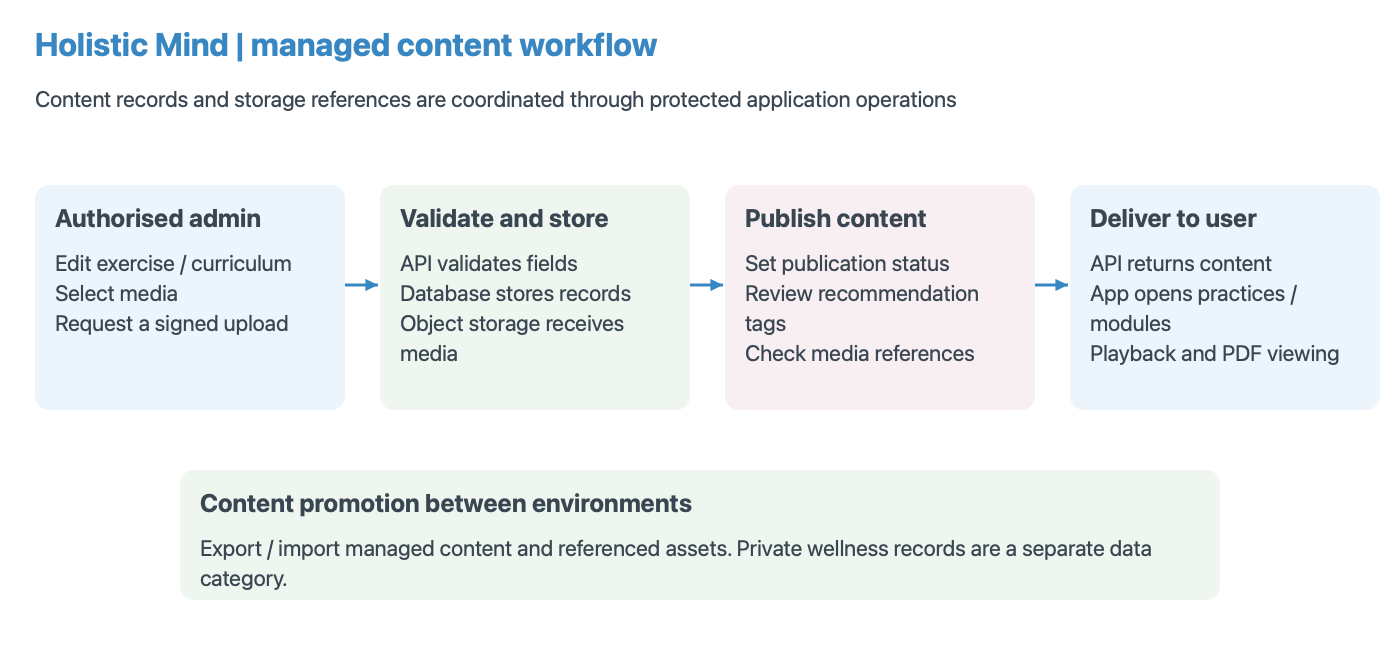
\includegraphics[width=\linewidth,height=0.62\textheight,keepaspectratio]{figures/content.png}
\caption[Content publication workflow]{Content publication workflow reconstructed from the implemented admin, API, and storage modules. A published record and usable media reference are distinct prerequisites for delivery.}
\label{fig:content}
\end{figure}
\FloatBarrier

\subsection{Screen-by-screen implementation}

The Home screen presents the daily check-in as the main action and follows it with suggested tools and progress information. The check-in stores six values: state, body, energy, stress, focus, and support. Comfort preferences are additional optional choices rather than a seventh inferred mental-health measurement. The final step can exclude self-touch, breath holds, head or eye scanning, and inward body scans. These choices apply to the stored check-in, so the user should not assume that they are permanent account-wide settings.

Explore provides independent access to exercise categories and available audio. A person can use it when no recommendation has been generated or when they prefer another activity. Exercise detail screens support the relevant guidance format, including timed breathing, guided material, and media playback. Recommendation feedback is associated with the returned practice context when available. Opening, starting, and completing are distinct events; none is treated as direct proof of benefit. Figure~\ref{fig:home_explore} shows earlier Home and Explore interfaces from the September progress review.

\begin{figure}[htbp]
\centering
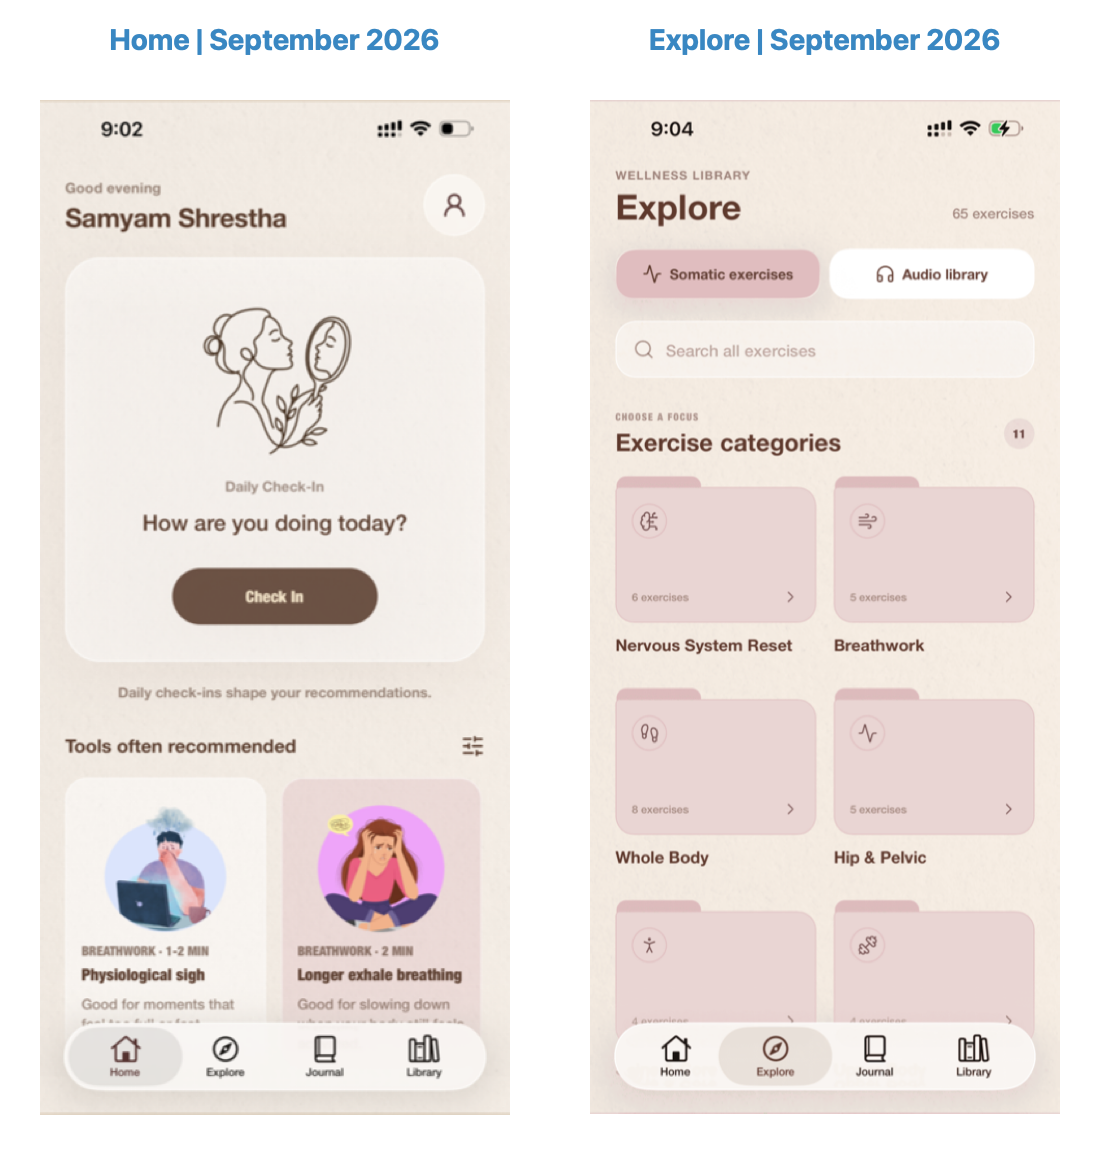
\includegraphics[width=\linewidth,height=0.62\textheight,keepaspectratio]{figures/home_explore.png}
\caption[Historical Home and Explore interfaces]{Historical Home and Explore interfaces reproduced from Shrestha's final progress review dated 2 September 2026. Catalogue counts and interface details describe that captured version.}
\label{fig:home_explore}
\end{figure}
\FloatBarrier

Journal supports prompted packs and free writing behind an unlock/\allowbreak{}setup gate. The free-writing editor manages title, text, attachments, save state, and unsaved changes. Navigation away from a draft asks whether it should be discarded. The current Journal security page centralises recovery and locking controls rather than placing a large control panel beneath every journal or history view. This refinement reduces visual clutter while keeping sensitive operations accessible through Profile.

Profile groups account details, password/\allowbreak{}security actions, preferences, reminders, and history. History brings together recorded check-ins, practice information, and reflections that can be decrypted while the vault is unlocked. The September screenshots show an earlier form of those screens (Figure~\ref{fig:history_profile}). The report uses them as development evidence, not as proof that every current control has been exercised on a physical device. The captions preserve that date so interface history does not become an implicit release certification.

\begin{figure}[htbp]
\centering
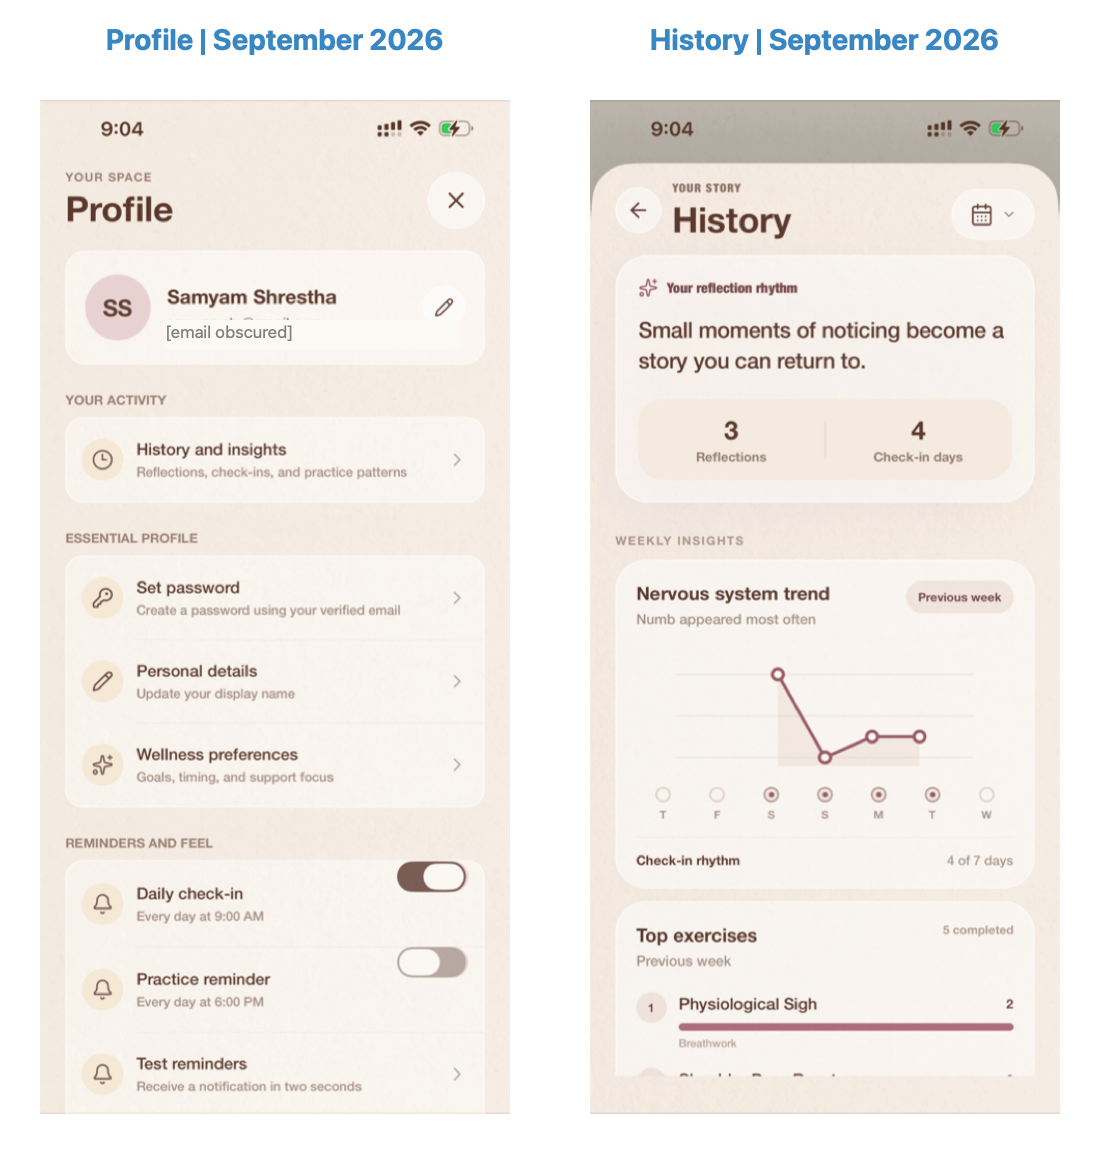
\includegraphics[width=\linewidth,height=0.62\textheight,keepaspectratio]{figures/history_profile.png}
\caption[Historical Profile and History interfaces]{Historical Profile and History screens from the 2 September 2026 progress review. The account email is obscured for presentation; journal security controls have since been reorganised.}
\label{fig:history_profile}
\end{figure}
\FloatBarrier

\subsection{Curriculum and audio implementation}

The learning Library is distinct from the short-practice catalogue. It uses courses, modules, and chapter records to organise longer material, with media and interactive chapter types defined in the backend. Section progress supports returning to a learning sequence. AudioPlayerContext provides a shared player state, and a compact player remains available across appropriate screens. This design avoids requiring the user to reopen the originating screen simply to pause a recording.

PDF viewing is handled separately from video and audio playback, with native and web implementations. The current code also includes interactive questions and multiple-choice content structures. Their availability allows the administrator to mix explanatory text, media, and participation within a course. It does not prove that the educational sequence has been assessed for learning effectiveness. A course can be technically navigable while still needing editorial review of its pacing, wording, and intended audience.

For usability, playback should remain predictable when navigating, receiving an interruption, or reopening the app. Those scenarios deserve native release testing because a web export cannot fully exercise platform audio behaviour. Likewise, successful PDF retrieval should be tested with large files, unsupported formats, and network errors. These priorities extend the final progress review's useful observation that apparently small interface defects can affect the overall experience.

\subsection{Authentication, provider configuration, and reminders}

Password hashing uses Argon2id in the current backend. Session handling, verification codes, and recovery actions are separate from journal recovery. Google sign-in requires matching native and backend client configuration as well as a reachable application API. The 3 October change record describes a simulator network failure caused by a stopped API and a new readiness check that presents a more specific failure message. It also states that a complete Google login still needs user retry. A configured provider should therefore not be described as end-to-end verified merely from source inspection.

Apple sign-in controls were removed from current login and signup screens on 3 October. Backend identity handling remains for existing Apple-linked accounts and account deletion. This corrects the earlier report's broader account-feature description. The final artefact should be documented at its current visible capability, with retained backend compatibility explained separately. It would be misleading to list Apple sign-in as a present mobile action simply because provider verification code remains in the repository.

Reminder scheduling uses Expo Notifications and local daily triggers when permission is granted. Current code schedules the daily check-in at 09:00 and practice at 18:00, with Android channel handling and a test reminder. The onboarding's preferred time is a separate stored value; its presence does not establish fully custom reminder scheduling. Web does not use these native local notifications. A release test should verify permission refusal, setting changes, cancellation on logout, and behaviour across device time changes.

\subsection{Journal media and atomicity}

Current source extends reflection beyond text through encrypted image and audio attachments. Media encryption binds the account, media identifier, key identifier, kind, content type, and entry association into authenticated data. This protects against substituting encrypted bytes into a different purpose or record. The journal context and attachment composer coordinate the draft, while the backend validates encrypted media and supports a combined entry-and-media operation. Encrypted user media is distinct from ordinary published exercise media.

The with-media endpoint uses a database transaction for the entry and related attachment records, allowing the server-side write to succeed or roll back as a unit. Client state still matters: recording, selecting an image, encryption, network transfer, and retry can fail before that transaction begins. The server's atomicity does not protect an unsaved local draft from being deliberately discarded. Tests should distinguish these stages rather than interpreting one transaction check as a complete attachment-workflow validation.

\subsection{Deployment evolution and release status}

The September final progress review reports a beta deployment using Railway, Vercel, and Cloudflare R2 alongside local Docker services. It also reports managed-content export/\allowbreak{}import without private user data. This is valuable historical evidence and should be retained. The report preparation did not independently query those deployments, inspect release logs, or exercise their live account operations. Later local encryption and security refinements therefore have their own validation and rollout boundaries.

A release of the present source requires coordinated backend schema, journal API, and native application versions. The latest encrypted clients expect envelope-based writes, while older plaintext clients are incompatible with that contract. Media configuration, API readiness, private recommender networking, email delivery, and native provider settings also require environment-specific checks. These are operational dependencies of the implemented system, not new features promised by this dissertation.

Figure~\ref{fig:evolution} summarises the main changes across the supplied reports and repository records. It shows the shift from a proposed Firebase-backed app to a relational multi-service platform, followed by stronger comfort and journal boundaries. The graphic is evidence of documented design evolution. It is not an independent verification of every historical deployment claim or an assertion that the proposed participant study has been completed.

\begin{figure}[htbp]
\centering
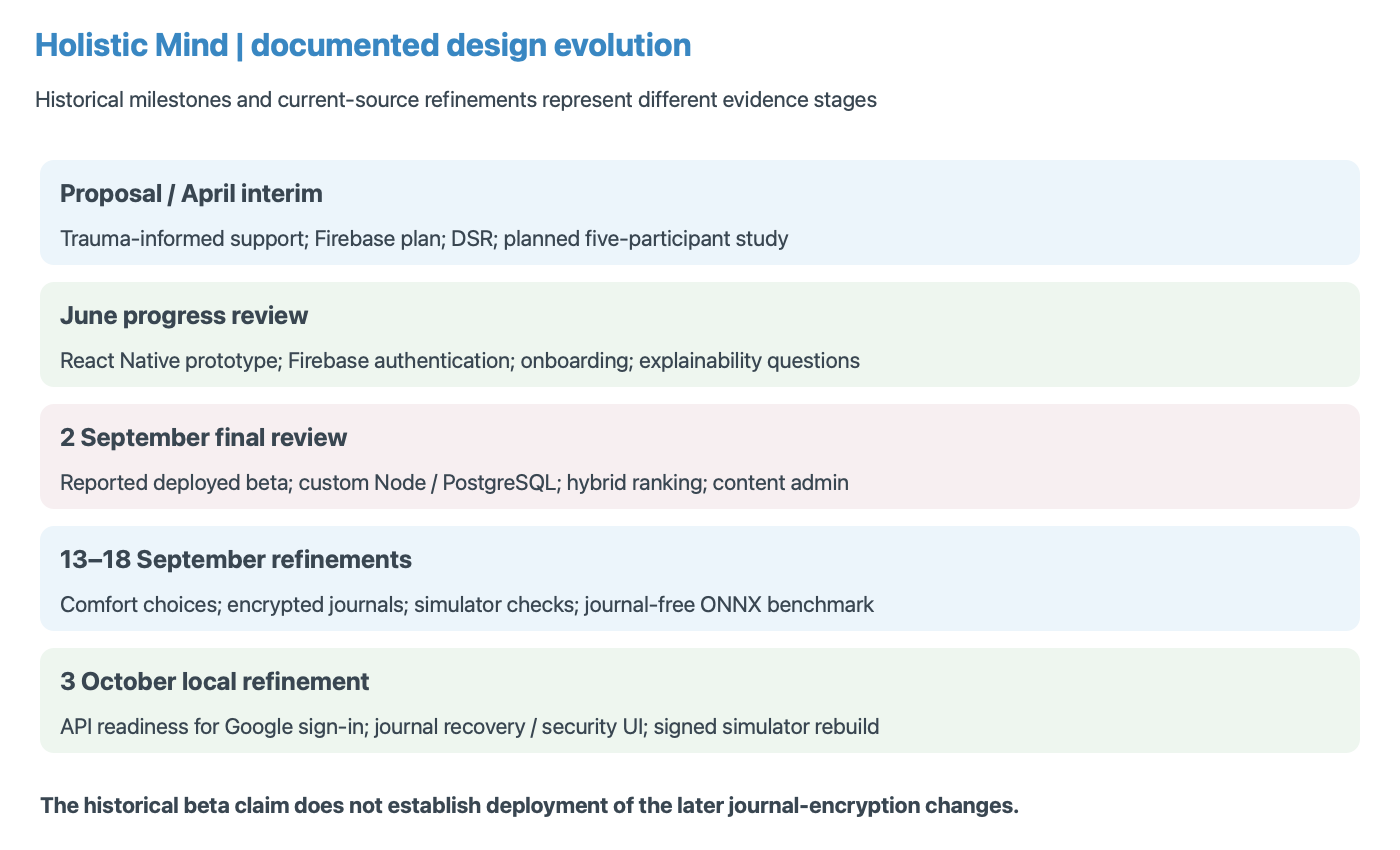
\includegraphics[width=\linewidth,height=0.62\textheight,keepaspectratio]{figures/evolution.png}
\caption[Evolution of the implemented design]{Project evolution across the April and June submissions, September final review, and later local refinements. Reported beta deployment and current encryption rollout are shown as distinct stages.}
\label{fig:evolution}
\end{figure}
\FloatBarrier
